\subsection{Recommendation}
\label{sec:Suggestion:Recommendation}

Wheras a \textsf{Change} concerns \textsf{MM}, a \textsf{Recommendation} describes
an action a methodologist may perform on \textsf{VT}. In our approach, we
issue a \textsf{Recommendation} for each \viewtype element impacted by a 
\textsf{Change}. We identified four kinds of \textsf{Action}s: a \textsf{REM}ove
\textsf{Action} indicates that a \viewtype element is no longer associated to an
\textsf{MM} element; an \textsf{ADD} suggests that a representation for a newly 
created \textsf{MM} element should be added in a \viewtype; an \textsf{UP}date
\textsf{Action} suggests to update a 


\begin{figure}[t]
    \centering
    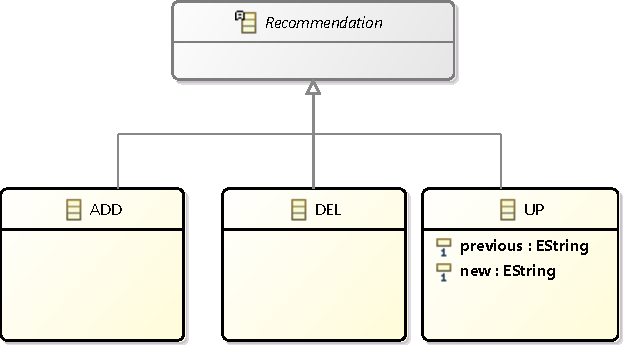
\includegraphics[width=0.8\columnwidth]{Recommendation.pdf}
    \caption{\textsf{Recommendation}s suggested after a \textsf{Change}
    e.g. in Step 1, \textsf{ADD} Attribute \textsf{name} in \textsf{Transition}}
    \label{fig:Recommendation}
\end{figure}